% Phylofriend User Guide
%
% For PDF output: pdflatex phylofriend.tex
% For HTML output: plastex pyhlofriend.tex
%
% For Graphics:
% Use PNG format to avoid problems with HTML conversion.
% Recommended size: < 13cm x 18cm (width x height).
% Recommended resolution: 300 dpi.
%
% Use fixed width instead of textwidth, so that plastex can
% recognize the graphics size. For example use
% 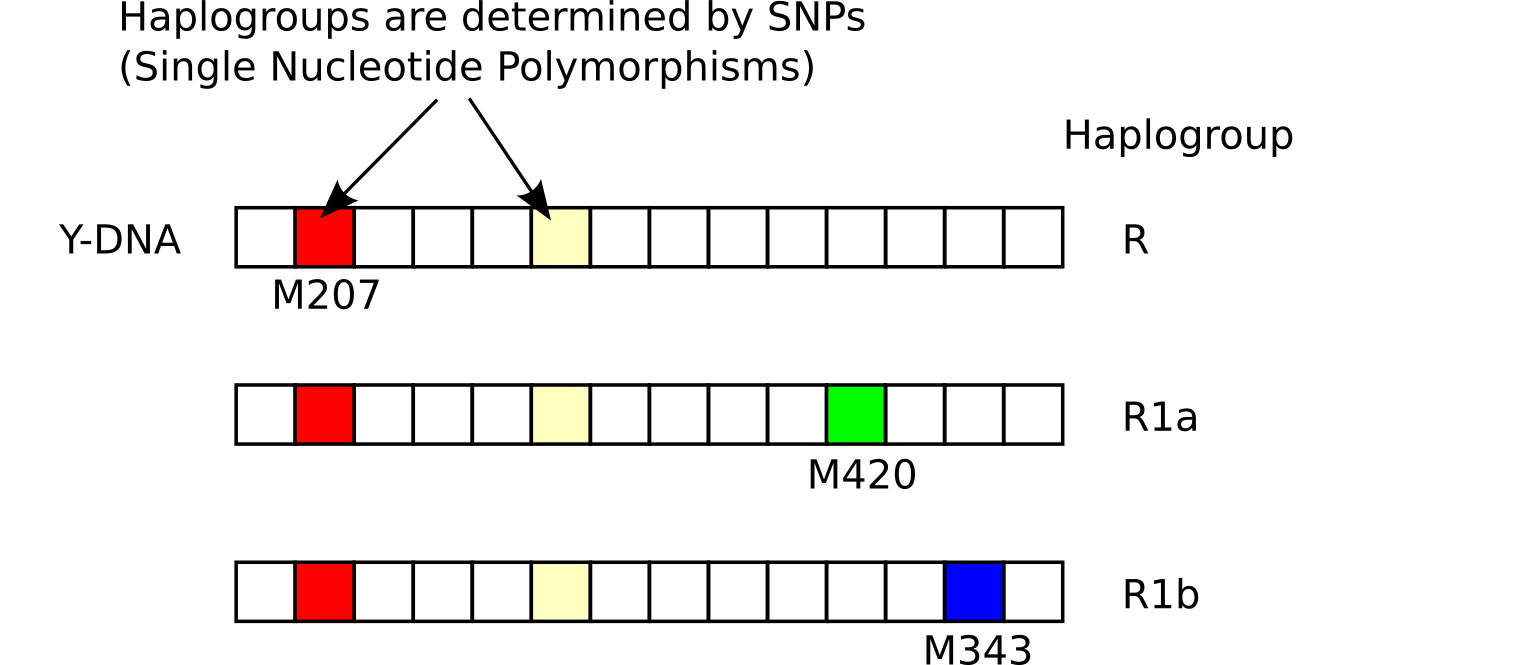
\includegraphics[width=13cm]{img/haplogroups.png}
% instead of
% 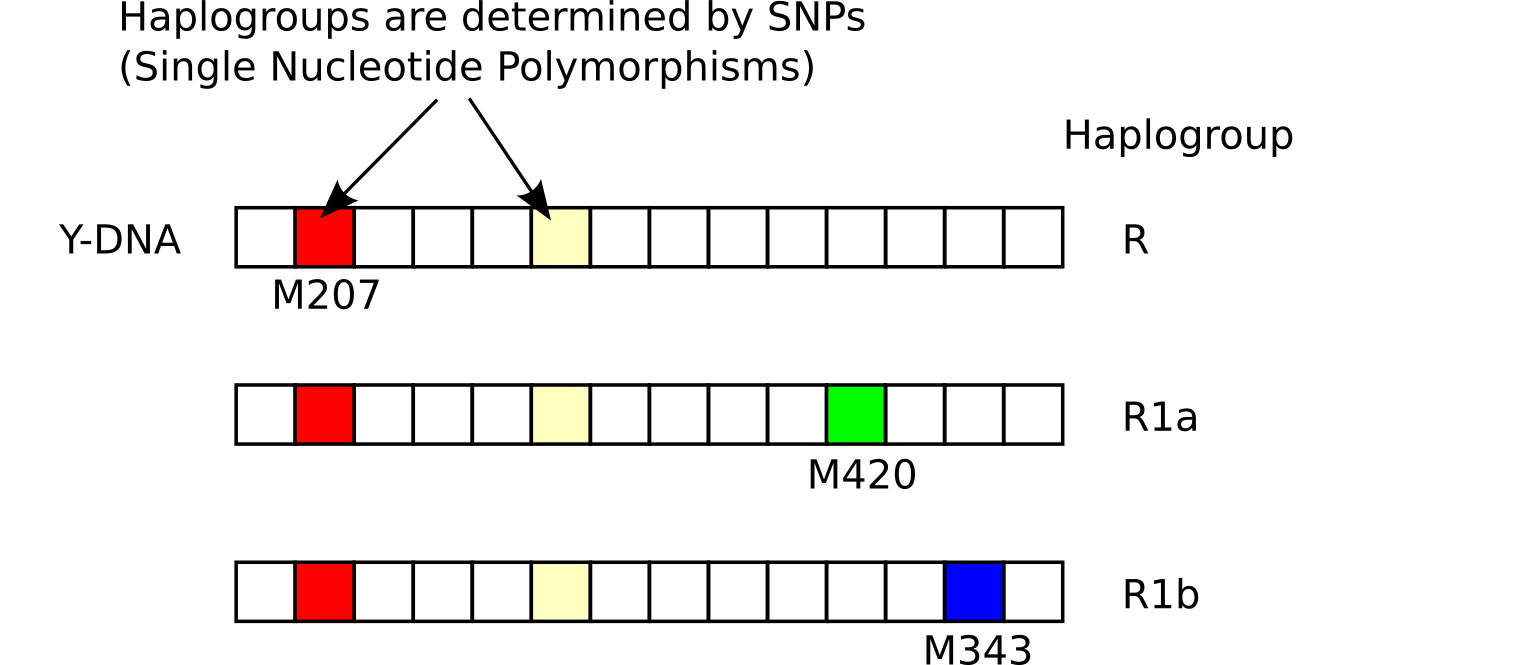
\includegraphics[width=\textwidth]{img/haplogroups.png}


\documentclass[12pt,a4paper]{article}
\usepackage[utf8]{inputenc}
\usepackage[english]{babel}
\usepackage[colorlinks=true, urlcolor=blue, linkcolor=blue]{hyperref}
\usepackage{graphicx}

\begin{document}
\begin{titlepage}

\title{Phylofriend User Guide}

\author{Dirk Struve\\
phylofriend at projectory.de\\
\href{https://github.com/yogischogi/phylofriend/}{https://github.com/yogischogi/phylofriend/}}
\date{\today}
\end{titlepage}
\maketitle

\tableofcontents
\section{Introduction}

Phylofriend's main purpose is to calculate genetic distances from
Y-DNA data. The results can be used as input for the
PHYLIP\cite{Phylip} program to create phylogenetic trees.

When I started creating phylogenetic trees I often found
myself in a difficult position. As a Linux user I was missing
some of the tools available under Windows. So I started
to write this program to fill in the gaps and make myself
comfortable again.

This does not mean that you can not use Phylofriend when
working under Windows or the Mac. But currently there is
no binary distribution available and you will probably face
a hard time installing Phylofriend and the associated programs.
So I only recommend this if you are an experienced user.

Phylofriend has some nice features. It can be used

\begin{itemize}
\item to create phylogenetic trees using the
	\href{http://evolution.genetics.washington.edu/phylip.html}{PHYLIP}\cite{Phylip}
	program. Y-STR values from Family Tree DNA projects can
	easily be imported.
\item as a programming library. Phylofriend is written in
	Google's \href{http://golang.org/}{Go} programming
	language. This language is not only suited to solve
	Google's large scale programming problems. It is also
	an excellent tool for part time programmers who have
	to concentrate on their projects (often students).
\item to extract Y-DNA data from Family Tree DNA projects
	and convert it into simpler text files that are
	better suited for further processing.
\item to automate phylogenetic tree creation. Phylofriend
	is a command line tool and this scares many people
	away. But if you have to repeat the same tasks over
	and over again you will eventually start to write some
	scripts and this is where command line tools come in
	handy.
\end{itemize}

I hope this program will be useful. Have a good time!

\vspace{1em} Dirk




\section{Installation}

This guide is mainly targeted towards persons who use Linux Mint
or other Linux versions of the Debian family. Some familiarity
with the use of Linux commands is assumed.

Currently there are no binary distributions available for
Windows or the Mac. Users of these operating systems can
use Phylofriend as well, but they will experience some
laborious installation work. The best way is to follow the
instructions provided on the
\href{http://golang.org/}{Go} home page and the
\href{http://evolution.genetics.washington.edu/phylip.html}{PHYLIP}
home page.

The following list applies to Linux users only:

\begin{enumerate}
\item Make sure that the Go programming language is installed.
	If not it can be installed by typing\\
	\texttt{sudo apt-get install golang}
\item Read the Go
	\href{http://golang.org/doc/install}{Getting Started}
	guide. Make sure to set your \emph{GOPATH} variable and
	include it in your \emph{PATH} so that Go programs can be
	found.
\item For the creation of phylogenetic trees install the
	PHYLIP program package by typing\\
	\texttt{sudo apt-get install phylip}
\item Fetch the Phylofriend program with\\
	\texttt{go get code.google.com/p/phylofriend}
\item Install the program with\\
	 \texttt{go install code.google.com/p/phylofriend}
\end{enumerate}


\section{Command Line Options}

Command line options may be given in arbitrary order.

\begin{description}
\item[-help] Prints available program options.
\item[-personsin] Filename or directory of files containing the
	persons' Y-STR values. If this is a single file it must contain
	results for multiple persons. The input file format is CSV
    (comma separated values) or text format.

	If a directory is provided for input it must contain multiple
	files in YFull format, each file containing the results for
	a single person. The person's ID is extracted from the filename.
\item[-labelcol] Number of the column that is used for labels
	when reading CSV files.
\item[-mrin] Filename of the mutation rates to use.
\item[-anonymize] If this is true persons' names are replaced by numbers.
\item[-modal] Creates modal haplotype and performs TMRCA calculation.
\item[-phylipout] Filename for the distance matrix that can be fed into
	the PHYLIP\cite{Phylip} program.
\item[-mrout] Filename for the output of the currently used mutation rates.
\item[-txtout] Filename for text output of persons and Y-STR values.
\item[-nmarkers] Uses only the given number of markers for calculations.
\item[-gentime] Generation time.
\item[-cal] Calibration factor.
\item[-reduce] Reduces the number of persons by the given factor
	 (for large numbers of samples).
\end{description}


\section{Examples}

\subsection{Create a Phylogenetic Tree}

\begin{enumerate}
\item Copy persons' data from a Family Tree DNA project website into
	a spreadsheet. If the Y-STR values do not appear properly try
	inserting them into the spreadsheet as unformatted text.
\item Save the spreadsheet in CSV (comma separated values)
	format, for example \emph{persons.csv}.
\item Start a terminal or command line interpreter and go
	to the directory where you stored \emph{persons.csv}.
\item Create a matrix of genetic distances by typing\\
	\texttt{phylofriend -personsin persons.csv -phylipout infile}
\item Use the PHYLIP program to create a tree in Newick format
	with\\
	\texttt{/usr/lib/phylip/bin/kitsch}\\
	You will need to answer some questions. Usually the
	default values are good enough. The results will be
	two text files, one named \emph{outtree} which contains
	the tree in Newick format and another one named
	\emph{outfile} which contains a more human readable
	description.
\item Create an image of the tree by typing\\
	\texttt{/usr/lib/phylip/bin/drawgram}\\
	Use \emph{outtree} as the input file name.
	The resulting tree will be stored in a file named 
	\emph{plotfile}.

	A nice alternative to visualize the tree is the use of the
	\href{http://www.trex.uqam.ca/index.php?action=newick&project=trex}
	{Trex}\cite{Trex}
	webserver. You can copy the contents of the file \emph{outtree}
	into the Trex window.
\end{enumerate}

If you do not specify a file containing mutation rates
Phylofriend will use average 37 marker values as default.
They can be found in \cite{Kly12}.


\subsection{Pimp Your Tree with Nicer Labels}

By default Phylofriend assumes that your persons input file's
first column contains a list of IDs. This is usually a Family
Tree DNA Kit number. The resulting tree is hard to read. Many
projects keep names in another column. You can access this 
column by using the \emph{labelcol} option. Suppose your second
column contains names. You can create a distance matrix with
names instead of IDs by typing

\noindent\texttt{phylofriend -personsin persons.csv -labelcol 2\\
-phylipout infile}

Due to compatibility issues with other programs the labels
must be 10 characters long and may only contain 8-bit
characters. Phylofriend will apply a transformation to
make sure that the requirements are fulfilled 
but the result is sometimes a bit strange.

You can also use the \emph{labelcol} option to create trees
that contain the origins of people or the haplogroups. Although
I strongly recommend to build trees only from people who
belong to the same haplogroup this is sometimes useful if
you want to know if different haplogroups are close on their
Y-STR values.

If you want to publish your tree you will often need to
protect the privacy of the members. This is what the
\emph{anonymize} option is for. By typing

\noindent\texttt{phylofriend -personsin persons.csv -phylipout infile -anonymize}

you will get a distance matrix where the names are replaced
by numbers.


\subsection{Use a Specific Set of Mutation Rates}

The first example uses Phylofriend's build in mutation rates
which are average values for the standard 37 marker test.
Phylofriend supports the use of arbitrary mutation rates by
the \emph{mrfile} option. The \emph{phylofriend/mutationrates}
directory contains some files with mutation rates. The average
mutation rates where taken from \cite{Kly12}.
If you like to compare on 67 markers you can use

\noindent\texttt{phylofriend -personsin persons.csv -phylipout infile\\
-mrin github.com/yogischogi/phylofriend/mutationrates/67-average.txt}


\subsection{Calibrate Your Data}

Mutation rates depend on the method applied to calculate
genetic distances and the sample populations used. Mutations
themselves occur by coincidence. Average mutation rates
often yield acceptable results but in most cases you will
have to calibrate your data especially if you want to
calculate in years.

Phylofriend provides two options for data calibration:
\emph{gentime}, the generation time in years and
\emph{cal} an additional calibration factor. Internally
they are just multiplied together but using two separate
factors seems more convenient for typical use cases.

The default value for the generation time is 25 years.
For time spans over the last few hundred years a generation
time of 30 years often yields better results. This can
be done by

\noindent\texttt{phylofriend -personsin persons.csv -phylipout infile\\
-gentime 30}

It is often difficult to calibrate data because you need a
reliable paper trail or a well defined historic event. If
you are lacking both you can try to apply Klyosov's statistical
method\cite{Kly09}. For large enough sample sizes this will
effectively reduce the statistical error but you will still
be left with an unknown systematical one.


\subsection{Count Mutations}

The \emph{phylofriend/mutationrates} directory contains
sets of mutation rates where all markers are set to 1.
This makes mutation counting easy but you will need an
additional little trick. Internally Phylofriend uses
average values. So it is possible to compare persons who
have tested on different sets of markers.

If you want to count mutations for example on a 37 marker
scale, you must multiply Phylofriend's internal results with
37. The easiest way to archive this is by misusing the
\emph{gentime} option. 

\noindent\texttt{phylofriend -personsin persons.csv\\
-mrin github.com/yogischogi/phylofriend/mutationrates/37-1.txt\\
-phylipout distancecount.txt -gentime 37}


\subsection{Extract Data from a Spreadsheet}

Spreadsheet data is often uncomfortable to handle, especially
if you want to write your own program and need to parse it.
For this purpose Phylofriend supplies the \emph{txtout}
option. It writes data to a text file in simplified form.

The easiest way to use it is

\noindent\texttt{phylofriend -personsin persons.csv -txtout persons.txt}

This extracts the data from \emph{persons.csv} and writes
it to \emph{persons.txt}. The first column of \emph{persons.txt}
contains the first column found in \emph{persons.csv}, usually
a set of IDs. The following columns contain the Y-STR values.
All columns are separated by tabs.

If you want to use another column you can use the
\emph{labelcol} option:

\noindent\texttt{phylofriend -personsin persons.csv -txtout persons.txt\\
-labelcol 2}

This extracts the second column from \emph{persons.csv} and
writes it to the first column of \emph{persons.txt}.

When using the \emph{txtout} option you will need to specify
how many Y-STR values are written to the text file. This is
done by \emph{nvalues}. Phylofriend will write the same number
of Y-STR values to each line. Missing values are written as
0, larger sets of Y-STR values are truncated. This is how to
write a full set of 111 markers:

\noindent\texttt{phylofriend -personsin persons.csv -txtout persons.txt\\
-nvalues 111}

















\section{Technicalities}

\subsection{Source Code Documentation}

To access the source code documentation point your
web browser to:

\begin{itemize}
\item \href{http://godoc.org/github.com/yogischogi/phylofriend}{http://godoc.org/github.com/yogischogi/phylofriend}
\end{itemize}

If you want to modify the source code it is best to
use \emph{godoc} locally on your computer.

\begin{enumerate}
\item If \emph{godoc} is not yet installed install it by typing\\
	\texttt{sudo apt-get install golang-go.tools}\\
	(Linux Mint)
\item Start the documentation web server with\\
	\texttt{godoc -http=:6060}
\item Point your web browser to \texttt{localhost:6060}.
\item Click on \emph{Packages} and search for \emph{phylofriend}.
\end{enumerate}

This will give you a nice overview of the internal program
documentation. You can also click on function names to browse
the source code.


\subsection{Mutation Model}

The two basic mutation models are the infinite alleles model
and the stepwise mutation model as explained by Bruce Walsh\cite{Wal02}.
Phylofriend uses a hybrid mutation model. Most markers are
calculated using the stepwise model, palindromic markers are
calculated as described in \cite{Can14}.

As the method for calculating the genetic distance is likely
to change with time please look at the internal program
documentation if you need more details.


\subsection{Mutation Rates}

The directory \emph{phylofriend/mutationrates} contains
files with predefined mutation rates.


\subsection*{Average Mutation Rates}

\begin{itemize}
\item 12-average.txt
\item 37-average.txt
\item 67-average.txt
\item 111-average.txt
\item 390-average.txt (experimental)
\item 500-average.txt (experimental)
\end{itemize}

In these files average mutation rates are used for the
corresponding set of markers. The mutation rates for 12,
37, 67 and 111 markers were taken from \cite{Kly12}.

The mutation rates for 390 and 500 markers are experimental.
They were derived by comparing YFull data of the
\href{http://yfull.com/groups/list/}{R1b-M343 (xP312 xU106) project}
to Family Tree DNA data from members of the
\href{https://www.familytreedna.com/groups/ht-3-5new/about/background}{R1b-M269 (P312- U106-) project}.
500-average.txt uses all known Y-STR markers that are
reported by YFull and Family Tree DNA. 390-average.txt leaves
out most of the palindromic markers. This marker set should
suffer less from saturation effects.

These mutation rates are useful for genealogical purposes.
During genealogical time frames (about 400 years) long time
stable markers rarely change. If such an event happens a
son may be immediately 1000 years away from his father in
terms of genetic distance. This is a correct result because
mutations are governed by coincidence and such events do
happen from time to time but it does not make much sense
to place a son far away from his family. So very stable
markers are purposely underweighted by using average
values.


\subsection*{12 Marker Single Mutation Rates}

\begin{itemize}
\item 12.txt
\item 37-12.txt
\item 67-12.txt
\item 111-12.txt
\end{itemize}

These files are basically the same as the average mutation
rates files but for the first 12 markers the mutation rates
are set per marker. This puts appropriate weight on
very stable markers. The mutation rates were taken from
Wikipedia\cite{Wiki-List_of_DYS_markers}. Although there
may be some doubt if data from Wikipedia can be trusted 
the first 12 markers are well known and they are in use
for a long time. So I just adopted them. The values should be
good enough for most purposes.

For each file the 12 marker mutation rates were multiplied
by a calibration factor so that their average value matches
that from the rest of the file.

These files are useful for deeper history or if you
observe changes on long time stable markers. If several
persons share the same value on a very stable marker they
probably belong together. So try these mutation rates to
see if the results make more sense than those obtained by
using average markers.


\subsection{CSV Input Format}

Example:

\begin{verbatim}
id1,"Dirk Struve",Germany,R1b-CTS4528,13,24,14,11,11-14,12,...
id2,"Pyl. O. Friend",Germany,R1b-CTS4528,13,24,14,11,11-14,...
\end{verbatim}

When importing a file in comma separated values format the
first column must contain IDs. An arbitrary number of columns
containing custom information may follow. The last columns
must contain at least 12 Y-STR values in Family Tree DNA order.
Rows containing comments are allowed.

Phylofriend will always try to parse the file as best as
it can.


\subsection{Text Format}

Example:

\begin{verbatim}
Dirk_Struv	13	24	14	11	11	14	12	12	12	12	14	28
Pyl._O._Fr	13	24	14	11	11	14	12	12	12	12	14	28
\end{verbatim}

The text format is a simplified format intended for easy
parsing and to work well with other programs. For compatibility
reasons the first column is exactly 10 characters long and
contains only non Unicode characters. Spaces are transformed into
underscores. The following columns contain Y-STR values
separated by tabs.


\subsection{YFull Format}

YFull files have a name like \emph{STR\_for\_YF01234\_20160222.csv}.
Each line of the file contains the result for a single marker and
sometimes additional information. Example:

\begin{verbatim}
DYS390;24;
DYS391;11;
DYS392;14;?
DYS393;13;
\end{verbatim}

Although the file is in CSV format, semicolons are used instead
of commas as separators. This may cause trouble if you try to
add additional results by hand. Phylofriend does not care if a
marker is provided multiple times. The last occurrence of a name
is considered the valid one. Thus you can add results from other
testing companies just by adding them to the end of the file.

Phylofriend tries to extract a person's ID from the filename. If
a file is named \emph{STR\_for\_YF01234\_20160222.csv}, the ID
will be \emph{YF01234}.

If you want to provide your own files, you do not need to stick
to the YFull naming convention. Just use the desired ID as a
filename like \emph{ID1234.csv}, but the file must end in 
\emph{.csv}.


\subsection{PHYLIP Format}

Example:

\begin{verbatim}
2
Dirk_Struv	0	0
Pyl._O._Fr	0	0
\end{verbatim}

The first line contains the number of entries. An entry
line contains an ID that is 10 characters long and contains
only non Unicode characters. Spaces are transformed into
underscores. The columns containing genetic distances
are separated by tabs. For readability reasons
Phylofriend writes only integers. If you need more precision
you can scale the distance by using the \emph{cal} option.








\raggedright
\begin{thebibliography}{bla}


\bibitem{Newick} James Archie, William H.E. Day, Wayne Maddison,
Christopher Meacham, F. James Rohlf, David Swofford, Joe Felsenstein,
\emph{\href{http://evolution.genetics.washington.edu/phylip/newicktree.html}
{The Newick Tree Format}}.
1986, Date accessed: 2014-08-06.

\bibitem{Can14} R. A. Canada,
\emph{\href{https://www.familytreedna.com/learn/y-dna-testing/y-str/infinite-allele-palindromic-markers/}
{How does the infinite allele comparison method work for palindromic markers?}}.
Family Tree DNA, 2014, Date accessed: 2014-08-07.

\bibitem{Phylip} Joe Felsenstein,
\emph{\href{http://evolution.genetics.washington.edu/phylip.html}
{PHYLIP, a free package of programs for inferring phylogenies.}}.
University of Washington, First version: 1980, Date accessed: 2014-08-06.

\bibitem{Kly09} Anatole A. Klyosov,
\emph{\href{http://www.jogg.info/52/files/Klyosov1.pdf}
{DNA Genealogy, Mutation Rates, and Some Historical
Evidence Written in Y-Chromosome, Part I:  Basic Principles and
the Method}}.
Journal of Genetic Genealogy, 5(2):186-216, 2009.

\bibitem{Kly12} Anatole A. Klyosov,
\emph{Ancient History of the Arbins, Bearers of Haplogroup R1b, from
Central Asia to Europe, 16,000 to 1500 Years before Present}.
Advances in Anthropology, Vol.2, No.2, 87-105,
\href{http://dx.doi.org/10.4236/aa.2012.22010}{doi:10.4236/aa.2012.22010}, 2012.

\bibitem{Trex} Alix Boc, Alpha Boubacar Diallo, Vladimir Makarenkov,
\emph{T-REX: a web server for inferring, validating and
visualizing phylogenetic trees and networks}.
Nucleic Acids Research (2012) 40 (W1): W573-W579.
\href{http://dx.doi.org/10.1093/nar/gks485}{doi: 10.1093/nar/gks485}, 2012. 

\bibitem{Wal02} Bruce Walsh,
\emph{\href{http://nitro.biosci.arizona.edu/ftDNA/models.html}
{Details on the various assumptions used in computing TMRCA}}.
Family Tree DNA, 2002, Date accessed: 2014-08-07.

\end{thebibliography}

\bibliography{literature}
\addcontentsline{toc}{section}{References}
\end{document}
